\section{Progettazione di una WSN}

	La progettazione di una WSN è influenzata dai seguenti fattori
	\begin{itemize}
		\item Reliability (o fault tolerance)
		\item Scalabilità
		\item Costi di produzione
		\item Limitiazioni hardware
		\item Topologia
		\item Ambiente applicativo
		\item Mezzo di trasmissione
		\item Consumo di potenza (o lifetime)
	\end{itemize}
	Analizziamo di seguito ogni parametro nel dettaglio
	
\subsection{Reliability}
	La \emph{tolleranza ai guasti} (\emph{fault tolerance}, \emph{reliability} o \emph{affidabilità}) è la capacità della rete di non interrompere il servizio anche in presenza di guasti.
	Un nodo può rompersi per perdita di potenza, danni fisici o interferenze ambientali ma questo non deve pregiudicare l'operatività di tutta la rete di sensori.
	
	L'affidabilità di un nodo sensore $K$ è modellata mediante una distribuzione di Poisson dalla seguente equazione
	\[ R_k(t) = e^{-\lambda_k t} \] 
	Essa fornisce la probabilità che sia verificata una rottura al tempo $t$,
	$\lambda_k$ rappresenta il tasso di rottura (failure rate).
	
	L'affidabilità di un broadcast range con $N$ nodi sensori è ottenuta nel seguente modo
	\[ R(t) = 1 - \prod_{k=1}^{N} [1 - R_k(t)] \]
	A seconda dell'affidabilità richiesta si possono variare i protocolli e gli algoritmi utilizzati.
	
\subsection{Scalabilità}
	Il numero di sensori in una regione può variare considerevolmente, da pochi e diverse migliaia.
	
	La densità dei sensori è il numero di nodi all'interno del \emph{radio range} $R$
	\[ \mu(R) = \frac{N \pi R^2}{A} \]
	dove $N$ è il numero di sensori all'interno della regione di area $A$, mentre $R$ è il range di trasmissione.

\subsection{Costi di produzione}
	Il costo deve essere basso.
	L'obiettivo è di raggiungere un prezzo inferiore a 1~\$/dispositivo, attualmente il costo varia tra \$25 e \$180.
	
\subsection{Topologia}
	Nella gestione della topologia di una sensor network si distinguono tre fasi
	\begin{enumerate}
		\item \textbf{Pre-deployment e deployment phase}\\
			I sensori possono essere gettati da un aeroplano (\emph{random deployment}) oppure possono essere disposti in modo organizzato (\emph{regualar deployment}).
			Nel caso di sensori mobili questi possono muoversi autonomamente e cercare aree di interesse, compensare  guasti nella rete oppure essere mossi da forze esterne come vento e acqua.
			
		\item \textbf{Post-deployment phase}\\
			Variazioni nella topologia possono verificarsi a seguito di cambiamenti di posizione, problemi di raggiungibilità (a causa di jamming, rumore, ostacoli, etc.), energia insufficiente, malfunzionamenti.
		
		\item \textbf{Re-deployment di nodi aggiuntivi}\\
	\end{enumerate}

\subsection{Mezzo trasmissivo}
	I dispositivi possono comunicare tramite onde radio, dispositivi ottici (infrarossi) o acustici.
	
\subsection{Consumo potenza}
	La sorgente di potenza (batteria) è molto limitata ed è il principale fattore che determina il tempo di vita del sensore; in molti scenari non è infatti possibile ricaricare le batterie, risulta quindi importante usare l'energia in modo parsimonioso.
	Spesso i dispositivi vengono dotati di due batterie, una batteria principale con il compito di alimentare il dispositivo ed una batteria tampone per l'invio dei dati raccolti prima del completo scaricamento.
	
	Da questo punto di vista assume importanza anche la scelta dei protocolli utilizzati per la trasmissione dei dati, si parla di \emph{Power Aware Communication Protocols} in quanto devono minimizzare la dimensione dei pacchetti e il numero di pacchetti scambiati.
	Alcuni studi hanno analizzato l'assorbimento energetico di ogni componente di un sensore e si è osservato che le fasi di trasmissione e ricezione risultano essere quelle più energivore (Figura \ref{fig:consumoEnergiaDispositivo}).
	
	\begin{figure}[h]
		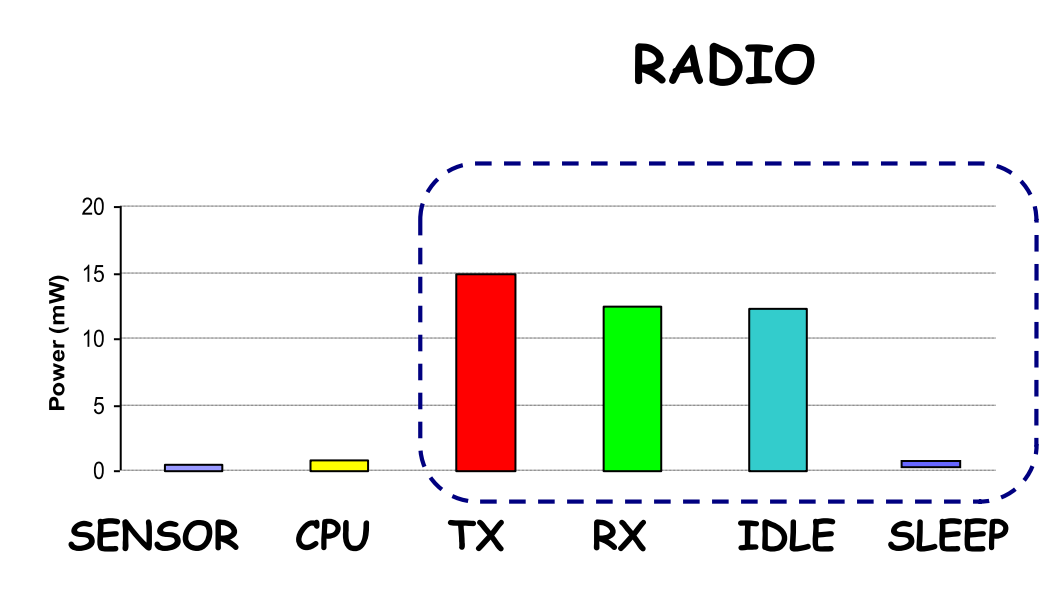
\includegraphics[width=\textwidth]{lez3/img/consumoEnergiaDispositivo.png}
		\caption{Consumo di energia per ogni componente del dispositivo}
		\label{fig:consumoEnergiaDispositivo}
	\end{figure}
	
	
	
	
	